\documentclass[12pt]{article}

%===============================
%
%          📦 Paquetes
%
%===============================

\usepackage[a4paper, top=2cm, bottom=2cm, left=2.5cm, right=2.5cm]{geometry}
\usepackage[spanish]{babel}
\usepackage[utf8]{inputenc}
\usepackage{amsmath}
\usepackage{multicol}
\usepackage{graphicx}
\usepackage{hyperref}
\usepackage{booktabs}
\usepackage{pgfplots}
\pgfplotsset{compat=1.18}
\usepackage{tikz}

\title{
  \vspace{2cm}
  \pagenumbering{gobble}
  
\includegraphics[width=5cm]{./assets/logo-utp.png} \\
  \vspace{1cm}
  \textbf{Universidad Tecnológica del Perú} \\
  \vspace{2cm}
  \textbf{Cálculo I} \\
  \vspace{1cm}
  \large \textbf{Taller 1}
}
\author{
  \textbf{Torres Vara, Mateo Nicolas} - \texttt{U24308542} \\
  \textbf{Zavala Padilla, Brayan Jhoseph} - \texttt{U20204620} \\
  \texttt{Sección 32384}
}



\begin{document}
\maketitle
\begin{center}

  Docente: Victor Johnny Papuico Bernardo

\end{center}

%======================================
%
%          📚 Inicio del documento
%
%======================================

\newpage
\section*{Ejercicio 1}
Dada las siguiente funciones
\begin{itemize}
  \item \[ f(x) = \log_3(x-4)+2 \]
  \item \[ f(x) = 3^{x-2}-5 \]
\end{itemize}

\begin{center}
\begin{minipage}{0.45\textwidth}
\begin{tikzpicture}
  \begin{axis}[
    axis lines=middle,
    xlabel={$x$},
    ylabel={$f(x)$},
    domain=0:14,
    samples=100,
    width=7cm,
    height=6cm,
    grid=both,
    xtick={0,1,3,5,7,9,11,13},
    ytick={0,1,2,3,4,5},
    ymin=0, ymax=5,
    xmin=0, xmax=14,
    title={$f(x) = \log_3(x-4)+2$}
  ]
  \addplot[blue, thick] {log10(x-4)/log10(3)+2};
  \addplot[blue, only marks, mark=*] coordinates {
    (4.33, 1)
    (5,2)
    (7,3)
    (13,4)
  };
  \addplot[domain=0:5, samples=2, dashed, thick, color=gray] ({4}, {x});
  \node[gray, right] at (axis cs:4,4) {$x=4$};
  \end{axis}
\end{tikzpicture}

\vspace{0.3cm}
\textbf{Dominio:} $x > 4$ \\
\textbf{Rango:} $(-\infty, \infty)$
\end{minipage}
\hfill
\begin{minipage}{0.45\textwidth}
\begin{tikzpicture}
  \begin{axis}[
    axis lines=middle,
    xlabel={$x$},
    ylabel={$f(x)$},
    domain=-2:6,
    samples=100,
    width=7cm,
    height=6cm,
    grid=both,
    xtick={-2,0,2,4,6},
    ytick={-12,-8,-4,0,4,8,12,16,20,24},
    ymin=-12, ymax=25,
    xmin=-2, xmax=5,
    title={$f(x) = 3^{x-2}-5$}
  ]
    \addplot[red, only marks, mark=*] coordinates {
      (3,-2)
      (4,4)
      (5,22)
    };
    \addplot[red, thick] {3^(x-2)-5};
    \addplot[domain=-2:6, samples=2, dashed, thick, color=gray] { -5 };
    \node[gray, below] at (axis cs:2,-5) {$y=-5$};
  \end{axis}
\end{tikzpicture}

\vspace{0.3cm}
\textbf{Dominio:} $(-\infty, \infty)$ \\
\textbf{Rango:} $(-5, \infty)$
\end{minipage}
\end{center}

\section*{Ejercicio 2}
Determine el dominio y la regla de correspondencia de las funciones $f - g$ y $\dfrac{f}{g}$

\vspace{-0.5cm}

\begin{center}
\[
\begin{array}{c@{\qquad}c}
  f(x) =
  \begin{cases}
    2x + 1, & x \in ]-5,3[ \\
    -x + 5, & x \in [3,10[
  \end{cases},  
  &
  g(x) =
  \begin{cases}
    1-x, & x \in [-10, 4] \\
    x-8, & x \in ]6, 15[
\end{cases}
\end{array}
\]
\end{center}

\vspace{0.5cm}

\begin{center}
\resizebox{\textwidth}{!}{%
\begin{tikzpicture}[yscale=1]
  \fill[gray!30] (-5,0) rectangle (3,0.5);   % overlap ]-5,3[
  \fill[gray!30] (3,0) rectangle (4,0.5);    % overlap [3,4]
  \fill[gray!30] (6,0) rectangle (10,0.5);   % overlap ]6,10[

  % Draw the number line
  \draw[thick] (-11,0) -- (16,0);

  % Tick marks and labels
  \foreach \x in {-10,-5,3,4,6,10,15}
    \draw[thick] (\x,0.08) -- (\x,-0.08);
  \foreach \x in {-10,-5,3,4,6,10,15}
    \node[below,font=\normalsize] at (\x,-0.08) {\x};

  % f(x) domain: ]-5,3[ and [3,10[
  \draw[blue,thick] (-5,1) -- (3,1);
  \draw[blue,thick] (3,1) -- (10,1);

  % Open/closed dots for f(x)
  \filldraw[white,draw=blue,thick] (-5,1) circle (1.5pt); % open
  \filldraw[white,draw=blue,thick] (3,1) circle (1.5pt); % open
  \filldraw[blue] (3,1) circle (1.5pt); % closed
  \filldraw[white,draw=blue,thick] (10,1) circle (1.5pt); % open

  % g(x) domain: [-10,4] and ]6,15[
  \draw[red,thick] (-10,0.5) -- (4,0.5);
  \draw[red,thick] (6,0.5) -- (15,0.5);

  % Open/closed dots for g(x)
  \filldraw[red] (-10,0.5) circle (1.5pt); % closed
  \filldraw[red] (4,0.5) circle (1.5pt); % closed
  \filldraw[white,draw=red,thick] (6,0.5) circle (1.5pt); % open
  \filldraw[white,draw=red,thick] (15,0.5) circle (1.5pt); % open

  % Legends
  \node[blue,right,font=\normalsize] at (10.5,1) {$f(x)$};
  \node[red,right,font=\normalsize] at (15.5,0.5) {$g(x)$};
\end{tikzpicture}}
\end{center}

\vspace{-0.5cm}

\[
\begin{minipage}{0.45\textwidth}
\[
\begin{array}{l}
  \multicolumn{1}{c}{f-g} \\[18pt]
  x \in ]-5, 3[ \; \Rightarrow \; 2x + 1 - (1 - x) = 3x \\[18pt]
  x \in [3, 4] \; \Rightarrow \; -x + 5 - 1 + x = 4 \\[18pt]
  x \in ]6, 10[ \; \Rightarrow \; -x + 5 - (x - 8) = 13 - 2x
\end{array}
\]
\end{minipage}
\hfill
\begin{minipage}{0.45\textwidth}
\[
\begin{array}{l}
  \multicolumn{1}{c}{f / g} \\[18pt]
  x \in ]-5, 3[ - \{1\}\; = \; \dfrac{2x + 1}{1 - x} \\[18pt]
  x \in [3, 4]  - \{1\}\; = \; \dfrac{- x + 5}{1 - x} \\[18pt]
  x \in ]6, 10[ - \{8\}\; = \; \dfrac{- x + 5}{x - 8}
\end{array}
\]
\end{minipage}
\]




\vspace{1cm}



\section*{Ejercicio 3}
Grafique la siguiente función $f(x) = -10 \cos\left(\dfrac{\pi}{6}x\right) + 4$, para un solo periodo.

\[
\begin{array}{c c c c c c}
  \left|a\right| = -10 \quad & w = \dfrac{\pi}{6} \quad & \O = 0 \quad & T = \dfrac{2\pi}{w} = 12 \quad & s = 3 \quad & b = 4
\end{array}
\]

\[
\begin{minipage}{0.3\textwidth}
\[
\begin{array}{c|c}
  0  & -6 \\ \hline
  3  & -4 \\ \hline
  6  & -6 \\ \hline
  9  & -4 \\ \hline
  12 & -6
\end{array}
\]
\end{minipage}
\hfill
\begin{minipage}{0.65\textwidth}
\begin{tikzpicture}
  \begin{axis}[
      axis lines=middle,
      xlabel={$x$},
      ylabel={$f(x)$},
      xtick={0,3,6,9,12},
      ytick={-6,-4,-2,0,2,4,6,8,10,12,14},
      ymin=-8, ymax=16,
      xmin=-1, xmax=13,
      grid=both,
      width=10cm,
      height=8cm,
      domain=0:12,
      samples=100,
    ]
    \addplot[blue, thick] {-10*cos(deg((pi/6)*x)) + 4};

    \addplot[blue, only marks, mark=*] coordinates {
      (0,-6)
      (3,4)
      (6,14)
      (9,4)
      (12,-6)
    };
  \end{axis}
\end{tikzpicture}
\end{minipage}
\]

\newpage
\section*{Ejercicio 4}
\noindent Fairbanks es una ciudad de Alaska. Es una de las ciudades más al norte de los EE.UU. Mientras que Miami es una de las ciudades más al sur de los EE.UU. Se ha logrado modelar la cantidad de horas F de luz natural en Fairkans y Miami mediante las siguientes funciones:

\[
F(t) = 13 - 9 \cos\left(\dfrac{\pi}{6}t\right) \quad \text{y} \quad M(t) = 10 - 5 \cos\left(\dfrac{\pi}{6}(t)\right)
\]

\noindent respectivamente. Donde $t$ es el tiempo en meses, desde el inicio hasta el fin del año 2016. ¿Cada cuánto tiempo la cantidad de horas de luz natural se repite en cada ciudad? ¿Cuáles fueron las cantidades de horas de luz natural máxima y mínima en cada ciudad? Grafique las funciones.

\vspace{0.5cm}

\begin{center}
\begin{minipage}{0.22\textwidth}
\textbf{Fairbanks}\\
\[
\begin{array}{c|c}
  t & F(t) \\ \hline
  0  & 4 \\ \hline
  3  & 13 \\ \hline
  6  & 22 \\ \hline
  9  & 13 \\ \hline
  12 & 4
\end{array}
\]
\end{minipage}
\hfill
\begin{minipage}{0.5\textwidth}
\begin{tikzpicture}
  \begin{axis}[
      axis lines=middle,
      xlabel={$t$ (meses)},
      ylabel={Horas de luz},
      xtick={0,3,6,9,12},
      ytick={0,5,4,10,13,15,20,22},
      ymin=0, ymax=24,
      xmin=-1, xmax=13,
      grid=both,
      width=10cm,
      height=8cm,
      domain=0:12,
      samples=100,
      legend style={at={(0.5,1.05)},anchor=south, font=\small, cells={anchor=west}}
    ]
    \addplot[blue, thick] {13 - 9*cos(deg((pi/6)*x))};
    \addlegendentry{Fairbanks (línea)}
    \addplot[blue, only marks, mark=*] coordinates {
      (0,4)
      (3,13)
      (6,22)
      (9,13)
      (12,4)
    };
    \addlegendentry{Fairbanks (puntos)}

    \addplot[red, thick] {10 - 5*cos(deg((pi/6)*x))};
    \addlegendentry{Miami (línea)}
    \addplot[red, only marks, mark=*] coordinates {
      (0,5)
      (3,10)
      (6,15)
      (9,10)
      (12,5)
    };
    \addlegendentry{Miami (puntos)}
  \end{axis}
\end{tikzpicture}
\end{minipage}
\hfill
\begin{minipage}{0.22\textwidth}
\textbf{Miami}\\
\[
\begin{array}{c|c}
  t & M(t) \\ \hline
  0  & 5 \\ \hline
  3  & 10 \\ \hline
  6  & 15 \\ \hline
  9  & 10 \\ \hline
  12 & 5
\end{array}
\]
\end{minipage}
\end{center}

\[
\begin{array}{c c c c c c}
  \left|a\right| = 9 \quad & w = \dfrac{\pi}{6} \quad & \O = 0 \quad & T = \dfrac{2\pi}{w} = 12 \quad & s = 0 \quad & b = 13
\end{array}
\]
\[
\begin{array}{c c c c c c}
  \left|a\right| = 5 \quad & w = \dfrac{\pi}{6} \quad & \O = 0 \quad & T = \dfrac{2\pi}{w} = 12 \quad & s = 0 \quad & b = 10
\end{array}
\]

\subsection*{Conclusiones}
\begin{itemize}
  \item La cantidad de horas de luz natural se repite cada 12 meses en ambas ciudades.
  \item En Fairbanks, la cantidad máxima de horas de luz natural es 22 horas y la mínima es 4 horas.
  \item En Miami, la cantidad máxima de horas de luz natural es 15 horas y la mínima es 5 horas.
\end{itemize}


\newpage
\section*{Ejercico 5}
\noindent Dada la siguiente función $f(x) = 0.5(x-5)^2+3$, para $x < 5$. Determine, el dominio, rango y la gráfica de f , Determine si existe la función inversa de f . Si existe, determine la regla de correspondencia de $f^{-1}(x)$, su dominio y rango y su gráfica. Finalmente, use la composición para probar que $\left(f o f^{-1}\right)(x) = x$.
\begin{center}
\begin{minipage}{0.48\textwidth}
\[
\begin{aligned}
  f(x) &= 0.5(x-5)^2 + 3, \quad x < 5 \\
  y &= 0.5(x-5)^2 + 3 \\
  y - 3 &= 0.5(x-5)^2 \\
  2(y - 3) &= (x-5)^2 \\
  x - 5 &= \pm \sqrt{2(y - 3)} \\
  x &= 5 - \sqrt{2(y - 3)}
\end{aligned}
\]
\end{minipage}
\hfill
\begin{minipage}{0.48\textwidth}
\[
\begin{aligned}
  \dfrac{1}{2}(5-\sqrt{2(x - 3)}-5)^2 + 3 &= x \\
  \dfrac{1}{2}(\sqrt{2(x - 3)})^2 + 3 &= x \\
  \dfrac{1}{2}(2(x - 3)) + 3 &= x \\
  x - 3 + 3 &= x \\
  x &= x
\end{aligned}
\]
\end{minipage}
\end{center}

\begin{center}
\begin{tikzpicture}
  \begin{axis}[
      axis lines=middle,
      xlabel={$x$},
      ylabel={$f^{-1}(x)$},
      domain=3:15,
      samples=100,
      width=8cm,
      height=7cm,
      grid=both,
      xtick={3,5,7,9,11,13,15},
      ytick={-5,0,1,2,3,4,5},
      ymin=-5, ymax=5,
      xmin=2, xmax=15,
      title={$f^{-1}(x) = 5 - \sqrt{2(x-3)}$}
    ]
    \addplot[red, thick] {5 - sqrt(2*(x-3))};
    \addplot[red, only marks, mark=*] coordinates {
      (3,5)
      (4,3.586)
      (7,2.172)
      (11,1)
    };
    \node[red, above] at (axis cs:3,5) {$x=3$};
  \end{axis}
\end{tikzpicture}
\end{center}

\newpage
\section*{Ejercicio 6}
\begin{center}
  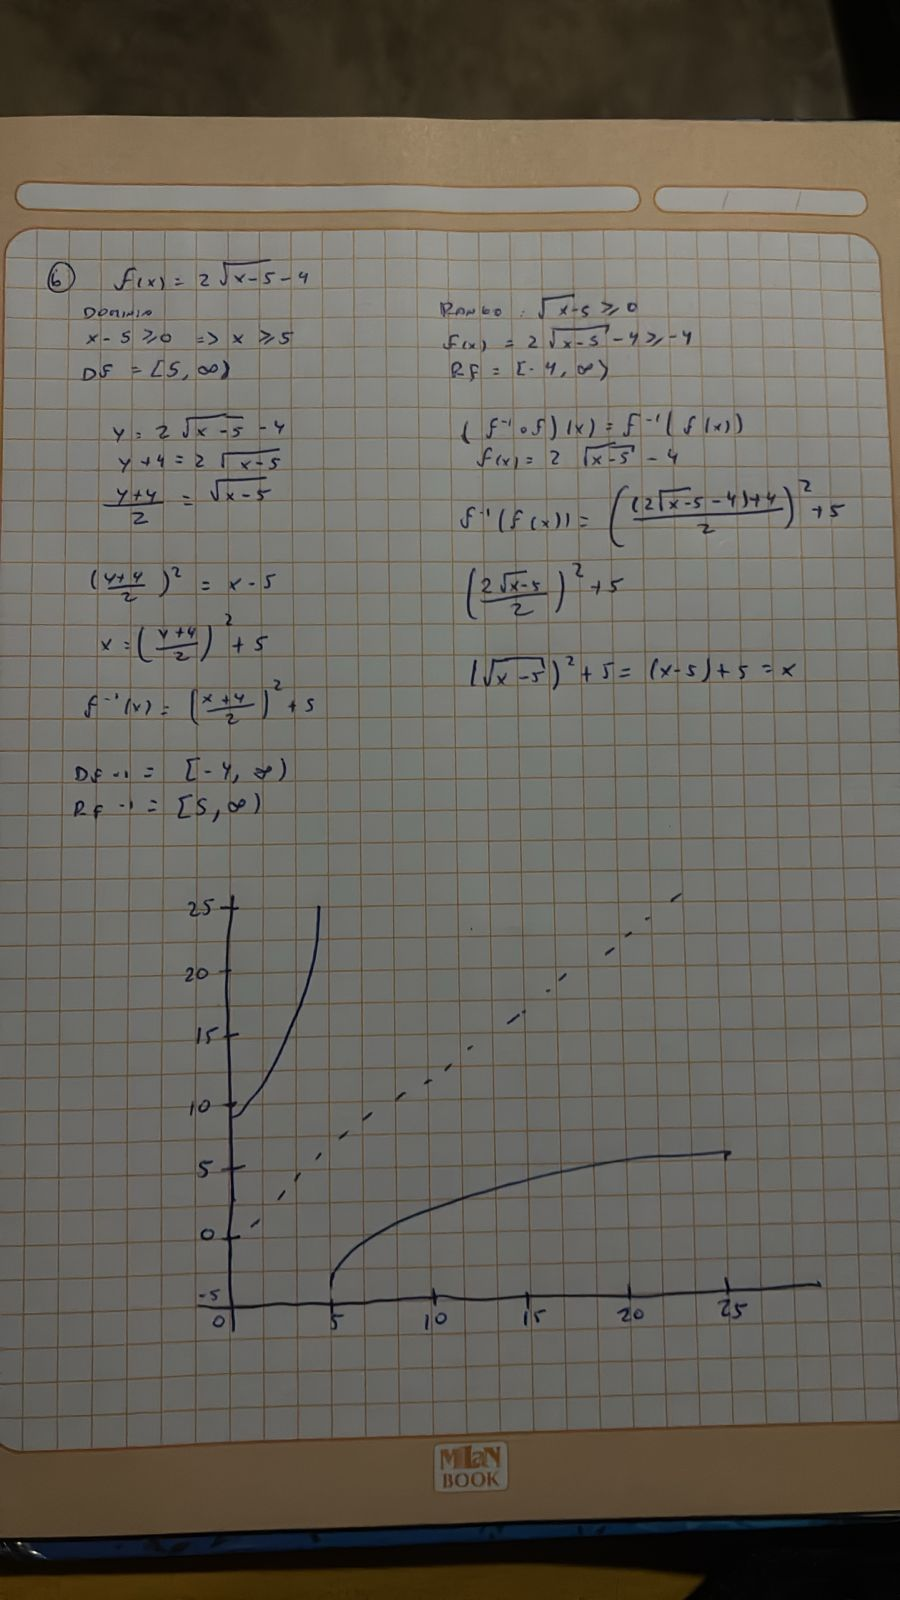
\includegraphics[width=0.8\textwidth]{./assets/ejercicio6.jpg}
\end{center}

\newpage
\section*{Ejercicio 7}
\begin{center}
  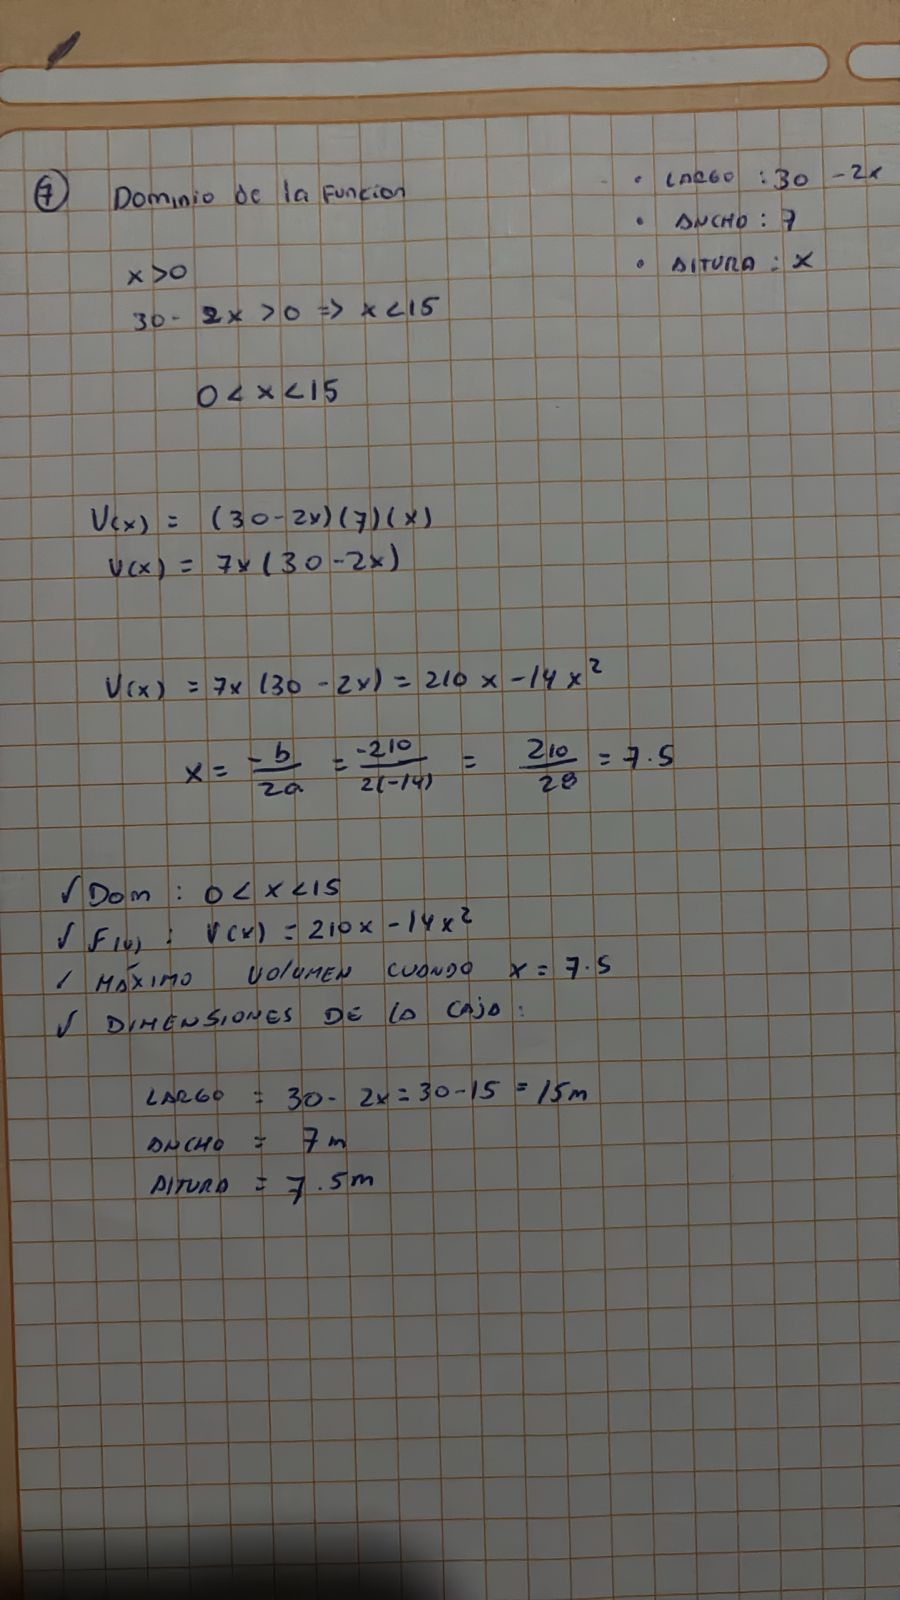
\includegraphics[width=0.8\textwidth]{./assets/ejercicio7.jpg}
\end{center}

\newpage
\section*{Recursos y créditos}

\begin{itemize}
    \item \textbf{Código fuente:} \href{https://github.com/MateoTVara/C08-CalculoI}{Repositorio GitHub - Cálculo I}
    \item \textbf{Carátula por:} \href{https://github.com/1nfinit0}{1nfinit0 en GitHub}
\end{itemize}

\end{document}